\chapter{Metoder}
\section{Litteratursøgning og metode}
\subsection{Litteraturstudie}
Undersøgelsens data og informationer er indhentet gennem litteraturstudier. Videnskabelig litteratur omhandlende videobaserede telesundhedsløsninger for hjemmepleje er søgt på følgende databaser: PubMed, Embase, CINAHL og Cochrane Library. Litteratursøgningsprocessen er udvidet til også at inkludere artikler identificeret ved kædesøgning i referencelister.\\
\begin{figure}[H]
\centering
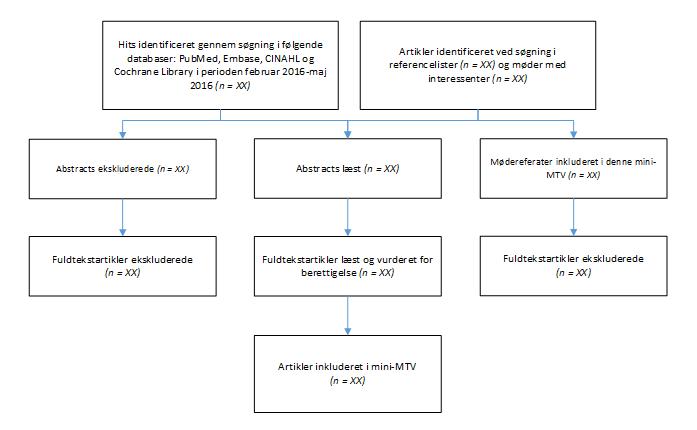
\includegraphics[width=1\textwidth]{Figurer/metode_flow.png}
\caption{\label{fig:metodeflow}Flowdiagram over  litteraturstudie. Flowdiagrammet angiver litteratursøgningsprocessen og identificerer antallet af ekskluderede og inkluderede artikler i MTV'en.}
\end{figure}

Emneord: Home Telemedicine, Telemedicine, Tele Care, Health Care, Tele Health Care.\\ \\
Ekskluderede artikler var telemedicinske problemstillinger vedrørende medicinsk behandling af patienter over distance, eksempelvis sårbehandling over skærm, hjemmemonitorering og telemedicinsk palliation. De inkluderede artikler omhandlede problemstillinger af telesundhedskarakter og havde fokus på virtuel hjemmepleje, eksempelvis medicinadministration og tilfredshedsundersøgelser. 
Nedenstående tabel viser inkusionskriterne:
\begin{table}[H]
\caption{Inklusionskriterier}
\label{tab:inklusionstabel}
\centering
\begin{tabularx}{\textwidth}{lX}
\hline
Populationer/deltagere & Patienter, borgere og sundhedsprofessionelle uanset diagnose eller sundhedsforhold
Søgningen blev begrænset til studier i patienters/borgeres eget hjem
Der var ingen aldersbegrænsning af populationer/deltagere\\ \hline
Indsatser             & Informations- og kommunikationsteknologier (IKT) på sundhedsområdet        \\ \hline
Sammenligninger             & Fysisk hjemmeplejebesøg og virtuel hjemmeplejebesøg          \\ \hline
Udfald             & Sundhedsrelaterede udfald (livskvalitet, patient-/borgertilfredshed), procesudfald (sundhedsprofessionelles tilfredshed, kvaliteten af pleje)          \\ \hline
\end{tabularx}
\end{table}

På baggrund af inklusions- og eksklusionskriterierne er antallet af artikler inkluderet i denne mini-MTV n = XX. Samtlige artikler er udenlandske, men er vurderet repræsentative for denne case, idet parametrene, som borgerafsnittet undersøger, er sammenlignelige med de udenlandske studier på området. En fuldstændig generalisering er ikke mulig, idet sundhedsforholdene varierer i de forskellige lande, så en fuldstændig sammenligning på tværs af landegrænser er ikke mulig. Dog er hensigten med resultaterne i borgerafsnittet ej heller at være generaliserbare, men i stedet at belyse borgernes reaktion på virtuel hjemmepleje i ’Pilotprojekt Videokommunikation’ fra Sundhedscenter Hadsten i Favrskov Kommune. Derfor er det i acceptabelt grad muligt at sammenligne og overføre resultater fra udenlandske studier til denne mini-MTV.

\subsection{Generel dataindsamling}
Data er endvidere indhentet gennem møder med forskellige interessenter – Appinux, Netplan Care og medarbejdere i Favrskov Kommune. Møderne har influeret på afgrænsningen af fokus, og på baggrund af disse møder er problemstillingen konkretiseret yderligere. Der er opnået et afgørende indblik i interessenters interesser i forbindelse med udbredelsen af virtuel hjemmepleje. Der er desuden indhentet viden om, hvorledes en kommune organiserer sig og særligt, hvad kommunal hjemmepleje er karakteriseret ved. På Favrskov Kommunes hjemmeside er der fundet oplysninger vedrørende hjemme- og sygepleje i Favrskov Kommune. Google i al almindelighed er ligeledes benyttet til indhentning af generel information om emnet telesundhed.

\subsection{Empirisk dataindsamling}
Med baggrund i de fokuserede spørgsmål har en stor del af fokus været på at belyse borgernes og sygeplejerskernes oplevelser og erfaringer med virtuel hjemmepleje. Det har derfor været nærliggende at supplere litteraturstudiet og den generelle dataindsamling med en kvalitativ interviewundersøgelse for netop at opnå en indgående og detaljeret viden herom.\\
I forbindelse med evalueringen af ’Pilotprojekt Videokommunikation’ blev der af Sundhedscenter Hadsten gennemført en lille kvalitativ evalueringsundersøgelse i form af strukturerede interviews med fire borgere og to sygeplejersker. Data fra denne interviewundersøgelse er indhentet og kritisk vurderet med henblik på anvendelse som empirisk datagrundlag i denne mini-MTV fremfor at igangsætte en ny empirisk videns indsamling.
\subsubsection{Diskussion af gyldigheden af den strukturerede interviewundersøgelse}
Interviews med høj struktureringsgrad har god anvendelse, når antallet af respondenter i undersøgelsen er få og genererer desuden en overskuelig datamængde sammenlignet med mindre strukturerede interviewundersøgelser. (KILDE – Bentes noter) ’Pilotprojekt Videokommunikation’ bestod af en begrænset gruppe borgere, sygeplejersker og øvrige medarbejdere. Antallet af mulige respondenter var altså få. Sammenholdt med den tids- og ressourcemæssige begrænsning i denne mini-MTV var designet af interviewundersøgelsen altså passende.\\ \\
Gyldigheden af de otte på forhånd udformede spørgsmål i interviewundersøgelsen blev vurderet høj, idet indholdet af disse svarede overens med denne mini-MTV’s ønske om at opnå et fyldestgørende indtryk af borgernes og sygeplejerskernes oplevelser med videoopkaldene i virtuel hjemmepleje i pilotprojektet. Spørgsmålene lignede således meget de pågældende spørgsmål, som en ny empirisk interviewundersøgelse ville have indeholdt.\\ \\
Samlet set er den indhentede interviewundersøgelse fra ’Pilotprojekt Videokommunikation’ fra Sundhedscenter Hadsten vurderet gyldig, hvorfor det er valgt at medtage denne. En vigtig essens at pointere ved anvendelsen af interviewundersøgelsen er, at denne ikke efterlader mulighed for generalisering. Formålet med at anvende kvalitativ metode i dette konkrete tilfælde har været at undersøge borgernes og sygeplejerskernes oplevelser med brugen af videoopkald som alternativ til konventionel fysisk hjemmeplejebesøg i forhold til Appinux-løsningen i ’Pilotprojekt Videokommunikation’ fra Sundhedscenter Hadsten. Formålet har ikke været at lave et generaliserbart studie med resultater, som direkte kan overføres til andre lignende cases. Ved at sammenholde den empiriske dataindsamling med relevant videnskabelig litteratur samt viden indhentet ved møder med interessenter har det været muligt at opnå en dybere forståelse for borgernes og sygeplejerskernes perspektiv. 

\section{Referencesystem}
I denne mini-MTV anvendes Vancouver som referencesystem. Kilder henviser til foregående linje og/eller afsnit, indtil foregående kildehenvisning. Ved henvisning til flere kilder anføres kilderne i parentes efter hinanden separeret ved et komma. Kildehenvisninger før en punktopstilling henviser til de følgende punkter. Citater fra interviews og andet er markeret med citationstegn, indrykket og skrevet i kursiv. Ved anvendelse af forkortelser skrives den fulde betegnelse første gang forkortelsen bruges[kilde:\url{http://library.au.dk/fileadmin/www.bibliotek.au.dk/Guides/Referencehaandtering/Litteraturhenvisninger_i_Vancouver.pdf}]

\section{Projektorganisation}
Projektgruppen har bestået af seks sundhedsteknologi ingeniørstuderende fra Aarhus ingeniørhøjskole. Fra projektets start blev der udvalgt en projektleder, Lise, der har til opgave at have det store overblik. Projektgruppen er endvidere blevet delt op i to, hvor den ene gruppe har haft ansvaret for borger- og organisations afsnittet, mens den anden gruppe har haft ansvaret for teknologi- og økonomi afsnittet. Indenfor hver gruppe er der blevet udvalgt en til hvert afsnit, som har det endelige ansvar. 

\section{Struktureret opbygning}
Denne mini-MTV rapport er opbygget ud fra MTV-tankegangen, hvor problemstillingen anskues ud fra fire hovedområder:\\
-	Teknologi/indsats\\
-	Patient/borger\\
-	Organisation\\
-	Økonomi\\
Skal vi have noget med om opbygningen af MTV’en eller er det ikke relevant? 


\begin{table}[h]
\begin{tabular}{lcccccc}
& Lise & Sara & Melissa &Jeppe &Mohamed & Jakob\\
\midrule
Projektleder &  X & & & & &\\
\midrule
Borger/Organisation &X & X & X & & &\\
Ansvaret for Borger & &  & X& & &\\
Ansvaret for Organisation & & X&  & & &\\
\midrule
Teknologi/Økonomi & & & & X &  X & X\\
Ansvaret for Teknologi & & & & X & &\\
Ansvaret for Økonomi & & & & & &X\\

\end{tabular}
\end{table} 

Hver torsdag klokken 10.15 har der været opsamlingsmøde, hvor alle grupper har fortalt om det de har fået lavet og hvad næste step er. Alle har til dette møde kunne komme med indvendinger og forslag til de forskellige afsnit.   
	

